% ********************************* HEADERS ***********************************
\documentclass{article}
\usepackage[top=.75in, bottom=.75in, left=.50in,right=.50in]{geometry}
\usepackage{fancyhdr}
\usepackage{titling}
\pagestyle{fancy}
\lhead{EECS 281 - Data Structures and Algorithms}
\rhead{\thepage}
\usepackage{color}
\usepackage{graphicx}
\newcommand{\heart}{\ensuremath\heartsuit}
\usepackage{listings}
\lstset{
  % language=C++,
  showstringspaces=false,
  basicstyle={\small\ttfamily},
  numberstyle=\tiny\color{gray},
  keywordstyle=\color{blue},
  commentstyle=\color{dkgreen},
  stringstyle=\color{dkgreen},
}
\usepackage[colorlinks,urlcolor={blue}]{hyperref}
%\setlength{\parskip}{1em}
\usepackage{parskip}
\usepackage{indentfirst}
\setlength{\droptitle}{-4em}
% \usepackage{concmath}
% \usepackage[T1]{fontenc}
\renewcommand{\theenumi}{\Alph{enumi}}
% ********************************* HEADERS ***********************************
\pagenumbering{gobble}
\begin{document}
\title{\textbf{EECS 281 Lab 8 - Fragmented Data Structures}}
\author{Due Tuesday, March 15th, 2017 at 11:59pm}
\date{}
\maketitle
\fancypagestyle{firststyle}
{
   \fancyfoot[L]{Written by Aaryaman Sagar for EECS 281 @ The University of
                 Michigan - Ann Arbor}
   \pagestyle{empty}
}
\thispagestyle{firststyle}

In this lab you will be using the transparent linked list from last lab to
finish writing a memory allocator to allocate memory on the heap!

\section{An untyped memory allocator}
You will be using the transparent list class you wrote in the previous lab to
write an untyped memory allocator very much like the C \texttt{malloc()}
function to allocate memory on the heap.

Memory allocators including the C++ \texttt{new} operator get memory on the
heap through function calls to the operating system.  You will be keeping
track of the memory available to you from all previous requests to the
operating system in a fragmented linked list.

A fragmented data structure is one that comprises of elements stored
discontinuously and possibly of different sizes.  The below two pictures
illustrate the difference between fragmented and non-fragmented data
structures.

\begin{figure}[!htb]
\centering
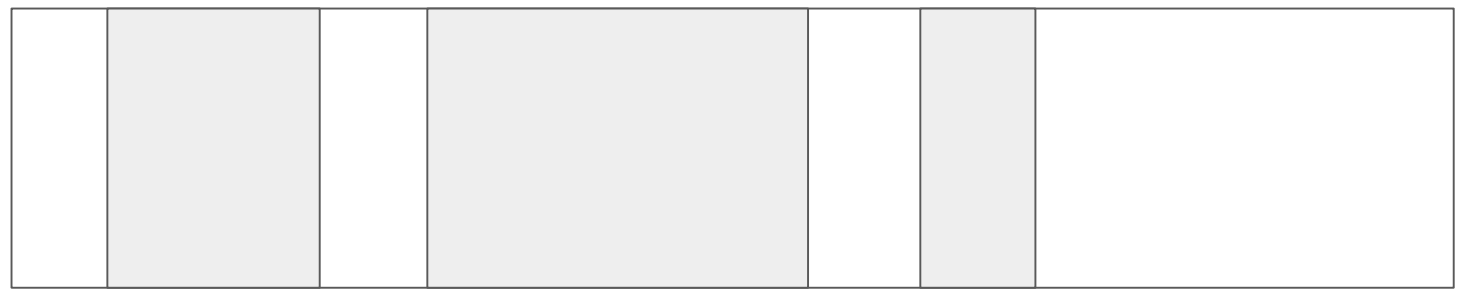
\includegraphics[height=3cm]{fragmented_memory}
\caption{Fragemented memory}
\end{figure}

\begin{figure}[!htb]
\centering
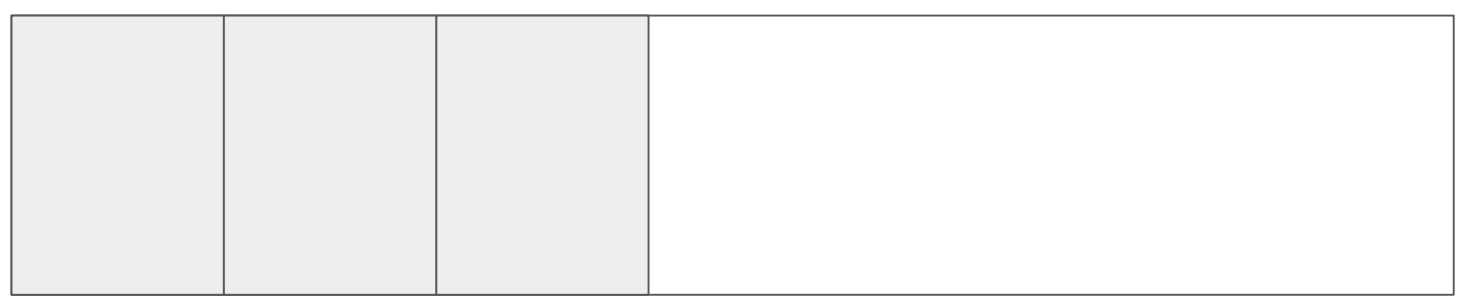
\includegraphics[height=3cm]{non_fragmented_memory}
\caption{Non fragemented memory}
\end{figure}

A memory request is served by returning a block of memory to the user for
usage.  This memory will be returned as a \texttt{void*} pointer which points
to a block of memory that is large enough to store the amount of data the user
has asked for.  The allocator keeps track of the memory segments and how large
each segment is by storing a header with the size information just before the
memory that is returned to the user.  This looks like so (with the grey
portion showing memory that can be used by the user, and the black showing
memory reserved for the header)

\begin{figure}[!htb]
\centering
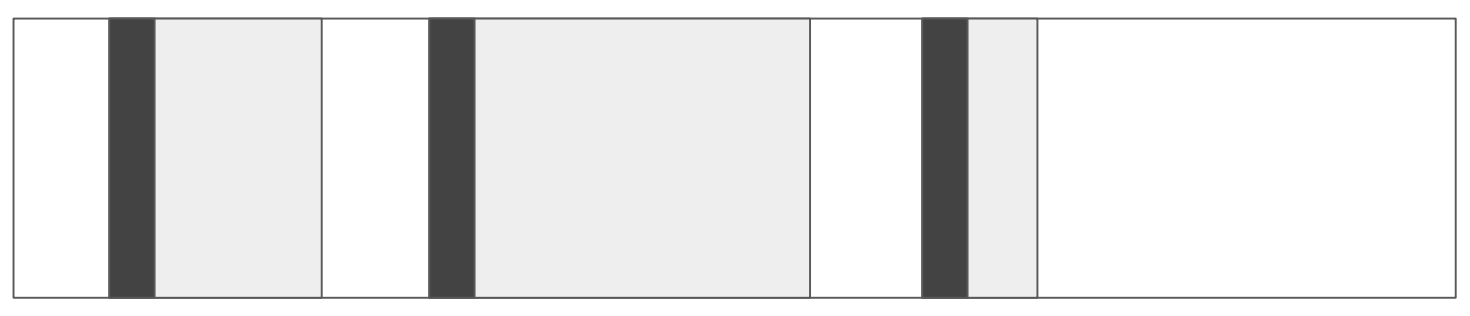
\includegraphics[height=3cm]{memory_storage}
\caption{Memory storage}
\end{figure}

In the above image, the pointer that will be returned to the user for usage
will start at the starting location of the grey area, and the header right
before that will contain the length of that grey area.  This way the allocator
knows how much memory each allocated block points to, so that if the
\texttt{free()} function is called on that memory, it can be put back into the
linked list of headers.

The linked list of headers will look like shown below, with each header
pointing to the next header in the logically increasing order or addresses
(for example here the first header on the left is at a lower location in
memory as compared to the second and the thirs and the second one is at a
lower location in memory as compared to the third)

\begin{figure}[!htb]
\centering
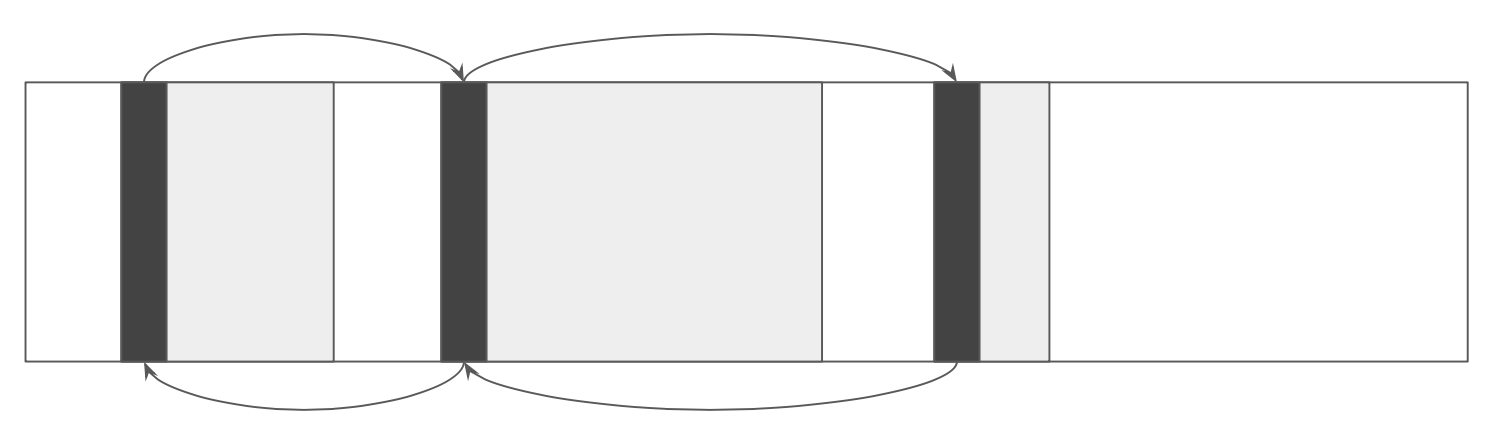
\includegraphics[height=3cm]{linked_list_headers}
\caption{Memory storage}
\end{figure}

When the user asks for memory, the block with the right amount of memory will
be taken out of the linked list and returned to the user, so for example if
the user asked for a really large portion of memory then the allocator can
return a portion of the second segment to the user.  Subsequently the free
list will be update to look like so

\begin{figure}[!htb]
\centering
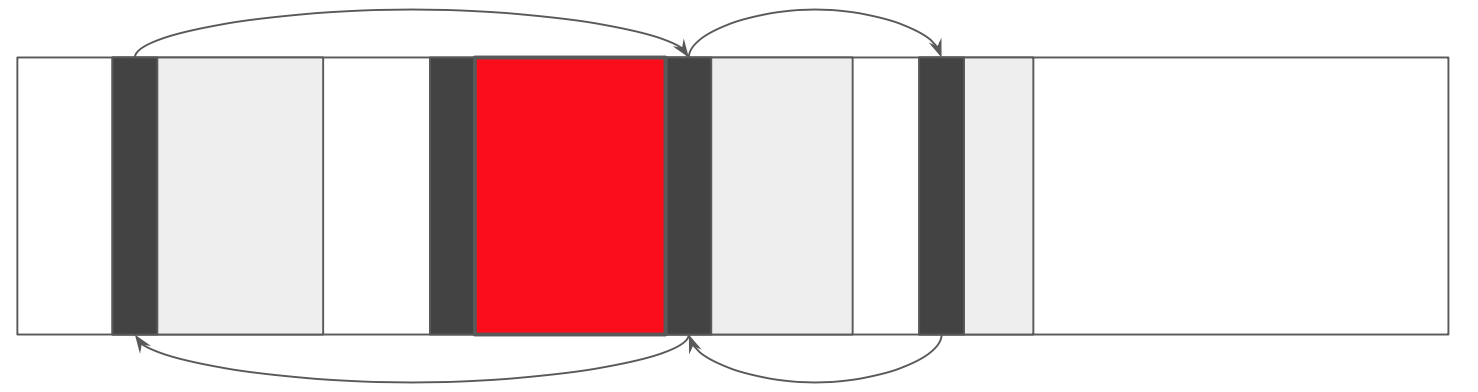
\includegraphics[height=3cm]{after_allocation}
\caption{After an allocation}
\end{figure}

And when the same memory is returned to the library via a call to
\texttt{free()} the free list will now look like as follows (the second and
third blocks will be coalesced back together)

\begin{figure}[!htb]
\centering
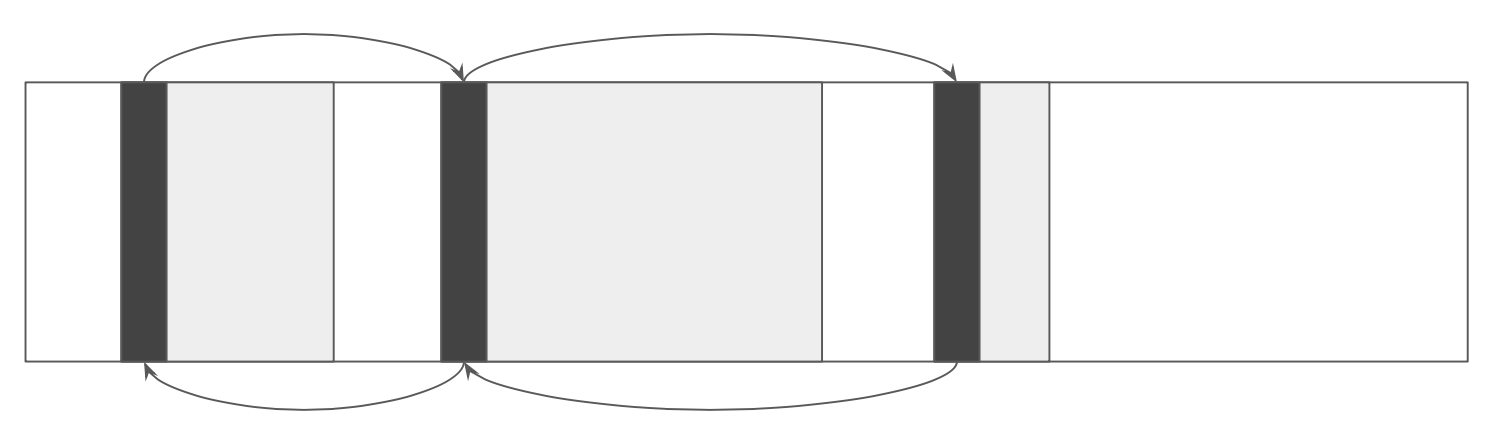
\includegraphics[height=3cm]{after_deallocation}
\caption{After a deallocation}
\end{figure}

\newpage
\subsection{Deliverables}

\newpage
\section{Submitting your work}
Please submit the implementation (\texttt{TransparentList.ipp}) file in a
tarball to the autograder, you can use the following command to generate the
tarball.
\begin{lstlisting}
    tar -czvf lab08.tar.gz TransparentList.ipp
\end{lstlisting}

\end{document}


